\chapter{Results, Auditability, and Security Analysis}
\begingroup
\justifying
\setlength{\parindent}{0pt}
\setstretch{2}
\setlength{\parskip}{0.5\baselineskip}
\titlespacing{\chapter}{0pt}{0pt}{0pt}
\titlespacing{\section}{0pt}{0pt}{0pt}

\section{Evaluation Methodology}

Evaluation focuses on three aspects:
\begin{itemize}
    \item \textbf{Functional correctness}: whether the system supports the intended election workflow end to end.
    \item \textbf{Verifiability}: whether invalid ballots and unsupported tally claims are rejected by contract verification.
    \item \textbf{Auditability and privacy}: whether voters can verify inclusion without revealing identity or ballot content.
\end{itemize}

Two complementary strategies are used: automated testing (contract and cryptographic unit tests) and workflow-based validation using the administrator and voter clients.

\section{Automated Verification Results}

The repository provides two automated verification layers.

\subsection{Smart Contract Integration Tests}

Hardhat tests validate:
\begin{itemize}
    \item voter registry permissions and one-vote enforcement;
    \item election lifecycle restrictions (Created/Active/Ended/Tallied);
    \item vote casting success path with Groth16 proof verification;
    \item invalid voting attempts (unregistered voter, duplicate vote, wrong phase);
    \item tally submission and state finalization behavior.
\end{itemize}

\subsection{Cryptographic Unit Tests}

Python tests validate BabyJubJub ElGamal primitives:
\begin{itemize}
    \item group arithmetic (associativity, identity, negation);
    \item key generation and serialization;
    \item encryption/decryption correctness across small message range;
    \item homomorphic addition correctness;
    \item one-hot encoding correctness for fixed candidate cardinality;
    \item bounded discrete-log recovery for tally extraction.
\end{itemize}

At the time of evaluation, the local test baseline was:
\begin{itemize}
    \item Hardhat tests: 36 passed.
    \item Python crypto tests: 43 passed.
\end{itemize}

These results support the claim that the prototype is reproducible and functionally coherent in controlled environments.

\subsection{Runtime and Reproducibility Snapshot}

To improve reproducibility, this dissertation records a concrete execution snapshot from the current repository revision.

\begin{table}[htbp]
\centering
\small
\caption{Automated Test Runtime Snapshot (Local Evaluation Run)}
\label{tab:runtime-snapshot}
\begin{tabular}{L{2.8cm} L{1.8cm} L{2.0cm} L{5.5cm}}
\toprule
Suite & Passed & Runtime & Command \\ 
\midrule
Hardhat contract/integration tests & 36/36 & about 15 s & \texttt{npm.cmd test} \\ 
Python cryptography unit tests & 43/43 & 21.31 s & \texttt{python -m pytest tests/ -q} \\ 
\bottomrule
\end{tabular}
\end{table}

Both suites completed with zero failures, for a combined 79 passing tests. This does not prove security in adversarial deployment, but it gives strong evidence that the implementation claims in Chapters 3--4 are executable and internally consistent on a fresh local run.

Table \ref{tab:evaluation-scenarios} provides a scenario-oriented view of what was validated and what evidence was observed.

\begin{table}[htbp]
\centering
\small
\caption{Evaluation Scenarios and Outcomes}
\label{tab:evaluation-scenarios}
\begin{tabular}{L{4.0cm} L{2.6cm} L{6.6cm}}
\toprule
Scenario & Result & Evidence \\
\midrule
Registered voter submits valid proof & Pass & Vote accepted and \texttt{EncryptedVoteCast} emitted. \\
Unregistered voter attempts to vote & Pass (rejected) & Contract revert on registration check before state change. \\
Duplicate vote attempt & Pass (rejected) & Contract revert through one-vote gating logic. \\
Tally finalization with proof & Pass & Result submission accepted after verifier call and status transition. \\
Receipt-based inclusion verification & Pass & Voter-side proof validation succeeds with matching receipt and bundle entry. \\
\bottomrule
\end{tabular}
\end{table}

\section{End-to-End Workflow Validation}

A practical end-to-end run proceeds:
\begin{enumerate}
    \item Administrator adds candidates and registers voter addresses.
    \item Election is started; voters generate ciphertexts and vote proofs in browser.
    \item Contract verifies vote proofs and emits encrypted vote events.
    \item Administrator aggregates encrypted ballots, decrypts totals, generates tally proof.
    \item Contract verifies tally proof and finalizes election with published Merkle root.
    \item Administrator exports \texttt{audit\_bundle.json}; voters verify inclusion using receipt.
\end{enumerate}

The key operational output is that a voter can validate inclusion without calling \texttt{getVoteRecord(address)}. This reduces address-based linkability and supports the project requirement of verifiable privacy.

\section{Commitment Merkle Auditability}

The audit design uses commitment leaves directly and derives internal nodes with Keccak. Deterministic event ordering ensures that independent auditors can reconstruct the same root given the same event set.

\subsection{Audit Bundle Content}

The exported audit bundle includes:
\begin{itemize}
    \item election identifier and chain metadata;
    \item Merkle root;
    \item commitment entries with indices and sibling proofs;
    \item transaction references for traceability.
\end{itemize}

\subsection{Anonymous Verification}

Using local receipt material, the voter client recomputes the commitment, locates matching entry, and verifies Merkle path. A successful verification implies that the commitment is included in the audited set whose root is published.

\section{Requirement Completion and Traceability}

Table \ref{tab:reqtrace} maps finer-grained requirements to concrete evidence.

\begin{table}[htbp]
\centering
\small
\caption{Fine-Grained Requirement Traceability}
\label{tab:reqtrace}
\begin{tabular}{L{4.0cm} L{2.6cm} L{6.6cm}}
\toprule
Requirement Item & Status & Evidence and Notes \\
\midrule
On-chain election lifecycle enforcement & Completed & Voting state machine and modifiers in \texttt{contracts/Voting.sol}. \\
Voter eligibility and one-vote rule & Completed & \texttt{contracts/VoterRegistry.sol} gates voting. \\
Ballot confidentiality (no plaintext on-chain) & Completed & Only ciphertext and commitment published; plaintext never stored. \\
Vote legality proof (range + one-hot) & Completed & \texttt{circuits/vote\_proof.circom} + verifier checks in \texttt{castVote}. \\
Ciphertext binding to vote proof & Completed (partial binding) & Circuit proves \texttt{ciphertextHash}; event payload binding not fully enforced (see Section 5.7). \\
Tally correctness proof (decryption) & Completed & \texttt{circuits/tally\_proof.circom} + verifier checks in \texttt{updateTallyResults}. \\
Merkle inclusion auditability & Completed & \texttt{frontend/lib/audit.js}, export bundle, verify inclusion. \\
Voter anonymity in verification & Completed (operational) & Receipt-based verification avoids address lookup; still relies on client privacy. \\
Production readiness & Not completed & Several hardening tasks remain (Section 5.7). \\
\bottomrule
\end{tabular}
\end{table}

\section{Security Analysis}

Figure \ref{fig:threat-model} summarizes the threat surface considered in this dissertation and the primary control layers used by the implementation.

\begin{figure}[htbp]
\centering
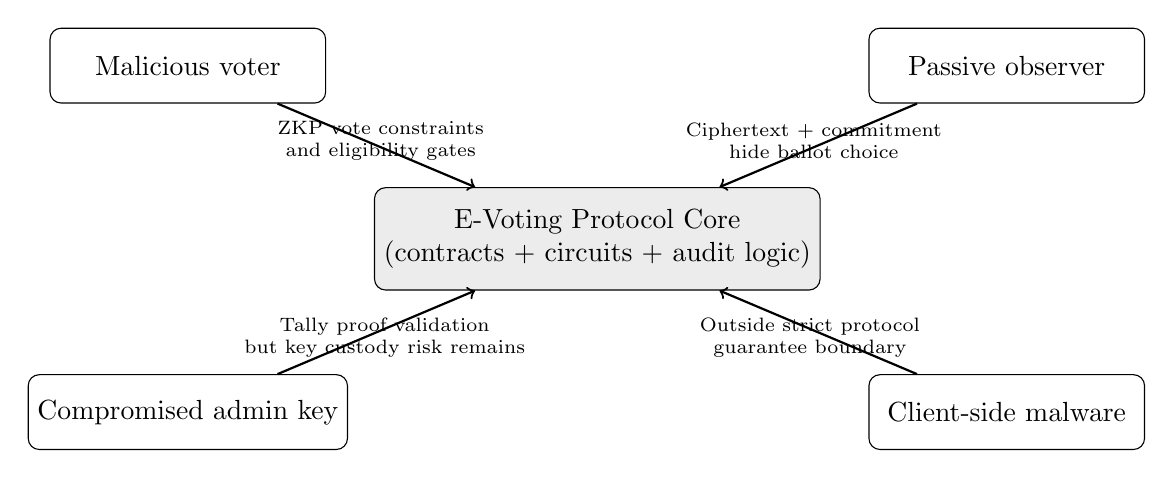
\begin{tikzpicture}[x=1cm,y=1cm]
    \node[draw, rounded corners, minimum width=5.2cm, minimum height=1.3cm, fill=gray!15, align=center] (core) at (0,0) {E-Voting Protocol Core\\(contracts + circuits + audit logic)};

    \node[draw, rounded corners, minimum width=3.5cm, minimum height=0.95cm] (t1) at (-5.2,2.2) {Malicious voter};
    \node[draw, rounded corners, minimum width=3.5cm, minimum height=0.95cm] (t2) at (5.2,2.2) {Passive observer};
    \node[draw, rounded corners, minimum width=3.5cm, minimum height=0.95cm] (t3) at (-5.2,-2.2) {Compromised admin key};
    \node[draw, rounded corners, minimum width=3.5cm, minimum height=0.95cm] (t4) at (5.2,-2.2) {Client-side malware};

    \draw[->, thick] (t1) -- (core);
    \draw[->, thick] (t2) -- (core);
    \draw[->, thick] (t3) -- (core);
    \draw[->, thick] (t4) -- (core);

    \node[font=\scriptsize, align=center] at (-2.75,1.25) {ZKP vote constraints\\and eligibility gates};
    \node[font=\scriptsize, align=center] at (2.75,1.25) {Ciphertext + commitment\\hide ballot choice};
    \node[font=\scriptsize, align=center] at (-2.7,-1.25) {Tally proof validation\\but key custody risk remains};
    \node[font=\scriptsize, align=center] at (2.7,-1.25) {Outside strict protocol\\guarantee boundary};
\end{tikzpicture}
\caption{Threat Model and Control Mapping}
\label{fig:threat-model}
\end{figure}

\subsection{Integrity Guarantees Achieved}

The system enforces:
\begin{itemize}
    \item lifecycle integrity through explicit state transitions;
    \item ballot validity through on-chain proof verification;
    \item tally proof verification before result finalization.
\end{itemize}

These properties meaningfully reduce risks common to centralized systems where validity and tally logic are opaque.

\subsection{Privacy Guarantees Achieved}

Ballot confidentiality is achieved by encryption and by ensuring that plaintext choices are never submitted to the chain. The commitment receipt is locally stored and does not directly reveal vote choice unless the salt is disclosed.

\subsection{Residual Risks}

Residual risks arise primarily from key custody and client environment. Even with cryptographic correctness, compromised endpoints can leak salts, candidate selection, or tamper with local witness generation. These are outside the guarantee boundary of the protocol.

\section{Outstanding Engineering Gaps and Their Impact}

Code review identified gaps that are important for full assurance:
\begin{itemize}
    \item \textbf{Result binding gap}: contract verifies tally proof but does not strictly bind the submitted integer result vector to all public signals used by the circuit. This can allow inconsistencies if external checks are not enforced.
    \item \textbf{Ciphertext event binding gap}: the emitted encrypted payload is not fully bound to on-chain stored ciphertext hash. If an attacker can influence event payload parsing or indexing, off-chain tally can be poisoned.
    \item \textbf{Audit root cross-check gap}: voter-side inclusion verification should compare bundle root with on-chain stored root to prevent acceptance of a self-consistent but unauthorized bundle.
    \item \textbf{Candidate cardinality mismatch}: circuits are compiled for three candidates while contract permits dynamic candidate count; this creates a mismatch risk if used incorrectly.
    \item \textbf{Merkle root mutability}: a direct root-update function exists without strict lifecycle gating; this increases governance attack surface.
\end{itemize}

These issues do not invalidate the prototype's educational value or end-to-end demonstration, but they prevent claiming full compliance with ``fully functional'' in a high-assurance sense.

Figure \ref{fig:assurance-gap} illustrates the current assurance profile: strong functional completeness, but a smaller unresolved hardening segment that must be closed before production use.

\begin{figure}[htbp]
\centering
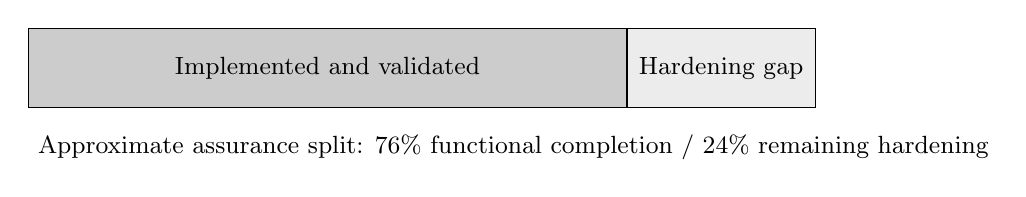
\begin{tikzpicture}[x=1cm,y=1cm]
    \draw[fill=gray!15] (0,0) rectangle (10,1.0);
    \draw[fill=gray!40] (0,0) rectangle (7.6,1.0);
    \draw[thick] (7.6,0) -- (7.6,1.0);
    \node[font=\small] at (3.8,0.5) {Implemented and validated};
    \node[font=\small] at (8.8,0.5) {Hardening gap};

    \node[anchor=west, font=\small] at (0,-0.5) {Approximate assurance split: 76\% functional completion / 24\% remaining hardening};
\end{tikzpicture}
\caption{Current Assurance Profile}
\label{fig:assurance-gap}
\end{figure}

\section{Threats to Validity}

The reported findings are subject to standard empirical-study validity limits:
\begin{itemize}
    \item \textbf{Internal validity}: tests are deterministic and mostly run on a local development chain; some network and wallet timing behaviors may be underrepresented.
    \item \textbf{Construct validity}: ``privacy'' in this dissertation primarily means ballot confidentiality plus receipt-based anonymous inclusion verification, not full coercion resistance.
    \item \textbf{External validity}: performance and usability observations may shift under larger electorates, different gas regimes, and different proof-artifact configurations.
    \item \textbf{Conclusion validity}: passing tests indicate consistency with encoded properties, but cannot by themselves establish absence of all protocol or implementation vulnerabilities.
\end{itemize}

To mitigate these threats, the dissertation combines protocol-level reasoning, cross-layer testing, and explicit gap documentation rather than relying on a single evidence source.

\section{Chapter Summary}

This chapter demonstrated that the implemented system is functionally complete as a verifiable privacy-preserving prototype and reproducible under automated testing. It also provided a requirement-grounded gap analysis that distinguishes current achievement from production-grade assurance.

\endgroup

